\section{Carrier Sense Multiple Access with Enhanced Collision Avoidance (CSMA/ECA)}\label{introProtocol}

CSMA/ECA~\cite{barcelo2008lba} is a fully distributed and collision-free MAC for WLANs. It differs from CSMA/CA in that it uses a deterministic backoff, $B_{\text{d}}=CW_{\min}/2$ after successful transmissions, where $CW_{\min}$ is the minimum contention window of typical value $CW_{\min}=16$. By doing so, contenders that successfully transmitted on schedule $n$, will transmit without colliding with other successful nodes in future cycles.

Collisions are handled as in CSMA/CA, which is described in Algorithm~\ref{alg:CSMA_CA}. In Algorithm~\ref{alg:CSMA_CA}, the node starts by setting the retransmissions counter and backoff stage to zero ($r\in[0,R]$ and $k\in[0,m]$ respectively, $m$ is the maximum backoff stage of typical value $m=5$, and $R$ is the retransmissions limit with typical value $R=m+1$), then generates a random backoff, $B$. When the Acknowledgement (\emph{ack}) for a sent packet is not received by the sender a collision is assumed. Upon collision, the involved nodes will double their contention window by incrementing their backoff stage in one and use a random backoff, $B\in[0,2^{k}CW_{\min}]$. This procedure is described between Line~\ref{collision} and~\ref{finalCollision} of Algorithm~\ref{alg:CSMA_CA}.

Algorithm~\ref{alg:CSMA_ECA} provides an explanation of CSMA/ECA's deterministic backoff mechanism, which main difference with CSMA/CA (and therefore with Algorithm~\ref{alg:CSMA_CA}) relies on the selection of a deterministic backoff after a successful transmission (compare Line~\ref{randomBackoff} in Algorithm~\ref{alg:CSMA_CA} with Line~\ref{deterministicBackoff} in Algorithm~\ref{alg:CSMA_ECA}). Figure~\ref{fig:BECA-example} shows an example of CSMA/ECA dynamics with four contenders.

\begin{algorithm}[ht!!!]
\While{the device is on}
{
  %\tcc{Initialize retransmission attempts.}
  $r \leftarrow 0$; $k \leftarrow 0$\;
  %\tcc{Initialize backoff counter.}
  $B \leftarrow \mathcal{U}[0,2^k{\rm{CW}_{min}}-1]$\;
  \While{there is a packet to transmit}{
    %\tcc{Initialize $a$.}
    \Repeat{($r = R$) or (success)}{
      %\tcc{First, backoff.}
      \While{$B>0$}{
        wait 1 slot\;
        $B \leftarrow B-1$\;
      }
      \colorbox{yellow}{Attempt transmission of 1 packet;}\\
      \If{collision}{\label{collision}
        %\tcc{Random backoff.}
        $r \leftarrow r+1$\;
        $k \leftarrow \min (k+1,m)$\;
        $B \leftarrow \mathcal{U}[0, 2^k {\rm{CW}_{min}} -1]$\;\label{finalCollision}
      }
    }
    $r \leftarrow 0$\;
    \colorbox{yellow}{$k \leftarrow 0$;}\\
	 \eIf{success}{
      %\tcc{Random backoff.}
      \colorbox{yellow}{$B \leftarrow \mathcal{U}[0,2^{k}{\rm{CW}_{min}}-1]$;}\\\label{randomBackoff}
    }
    {
      Discard packet\;
      $B \leftarrow \mathcal{U}[0,2^k {\rm{CW}_{min}}-1]$\;
    }
  }
  Wait until there is a packet to transmit\;
}
\caption{\small{CSMA/CA. $r$ indicates the number of retransmission attempts, while $R$ is the maximum retransmission attempts limit. When it is reached, the packet waiting for transmission is dropped.}}
\label{alg:CSMA_CA}
\end{algorithm}

\begin{algorithm}[ht!!!]
\While{the device is on}
{
  $r \leftarrow 0$ ; $k \leftarrow 0$\;
  $B \leftarrow \mathcal{U}[0,2^k{\rm{CW}_{min}}-1]$\;
  \While{there is a packet to transmit}{
    %\tcc{Initialize $a$.}
    \Repeat{($r = R$) or (success)}{
      %\tcc{First, backoff.}
      \While{$B>0$}{
        wait 1 slot\;
        $B \leftarrow B-1$\;
      }
      \colorbox{yellow}{Attempt transmission of 1 packet;}\\
      \If{collision}
      {
        %\tcc{Random backoff.}
        $r \leftarrow r+1$\;
        $k \leftarrow \min (k+1,m)$\;
        $B \leftarrow \mathcal{U}[0, 2^k {\rm{CW}_{min}} -1]$\;
      }
    }
    $r \leftarrow 0$\;
    \colorbox{yellow}{$k \leftarrow 0$;}\\
    \eIf{success}{
      %\tcc{Random backoff.}
      \colorbox{yellow}{$B_{d} \leftarrow (2^{k}{\rm{CW}_{min}})/2-1$\;}\label{deterministicBackoff}\\
	 $B \leftarrow B_{d}$\;
    }
    {
      Discard packet\;
      $B \leftarrow \mathcal{U}[0, 2^k {\rm{CW}_{min}}-1]$\;
    }
  }
  Wait until there is a packet to transmit\;
}
\caption{\small{CSMA/ECA.}}
\label{alg:CSMA_ECA}
\end{algorithm}


\begin{figure*}[tb]
\centering
  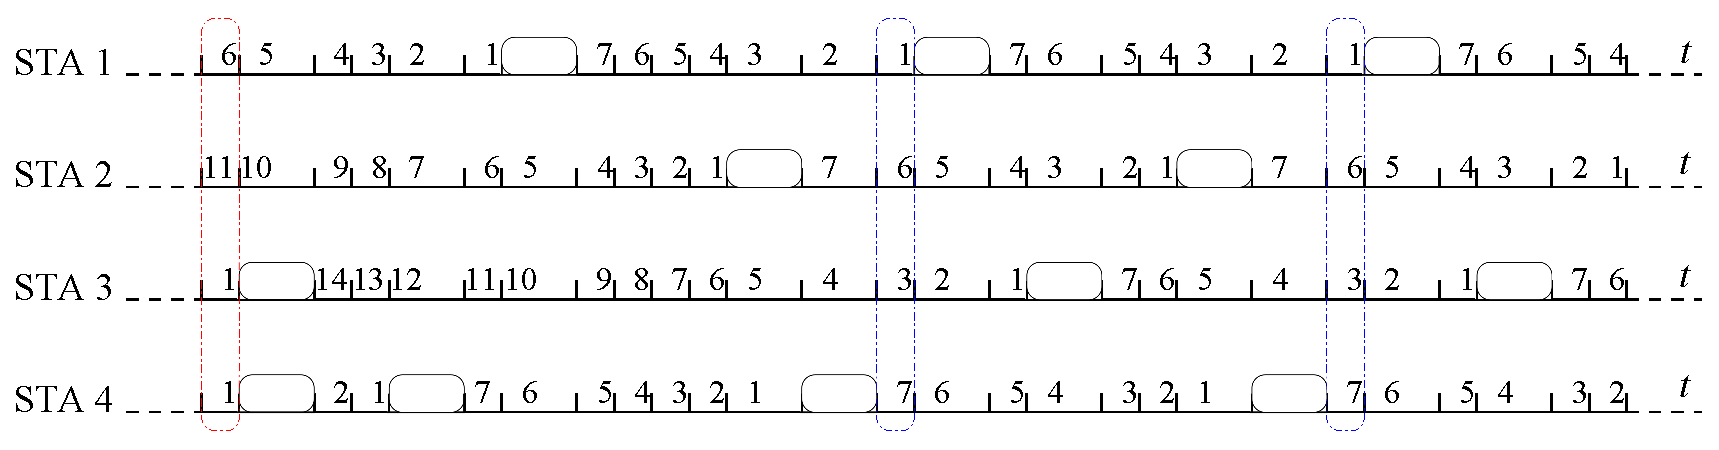
\includegraphics[width=0.8\linewidth]{figures/basicECA.eps}
  \caption{An example of the temporal evolution of CSMA/ECA in saturation}
  \label{fig:BECA-example}
\end{figure*}

In Figure~\ref{fig:BECA-example}, the \emph{STA-\#} labels represent stations willing to transmit. The horizontal lines represent a time axis with each number indicating the amount of empty slots left for the backoff to expire. Stations willing to transmit begin the contention for the channel by waiting a random backoff, $B$. The first outline highlights the fact that stations STA-3 and STA-4 will eventually collide because they have selected the same $B$. After recomputing the random backoff, STA-4's attempt results in a successful transmission, which instructs the node to use a deterministic backoff, $B_{\text{d}}=7$ in this case. By doing so, all successful STAs will not collide among each other in future cycles.

Collision slots being orders of magnitude larger than empty slots degrade the network performance. When CSMA/ECA builds the collision-free schedule all contenders are able to successfully transmit more often, increasing the aggregated throughput beyond CSMA/CA's. Figure~\ref{fig:BECA}, \textcolor{red}{shows the average aggregated throughput of CSMA/ECA, CSMA/CA and two of the collision-free protocolos presented in Section~\ref{relatedWork}, namely L-ZC and L-MAC~\cite{L_MAC}}.

%shows the achieved throughput of CSMA/ECA and CSMA/CA, alongside the Jain's Fairness Index (JFI)~\cite{JFI}.

\begin{figure}[tb]
\centering
  \includegraphics[width=0.7\linewidth, angle=-90]{figures/tonFigs/DCF-v-ECA-TON.eps}
  \caption{CSMA/ECA example in saturation: throughput (simulation parameters can be found in Section~\ref{simulations})}
  \label{fig:BECA}
\end{figure}

Referring to Figure~\ref{fig:BECA}, CSMA/ECA is able to achieve an aggregated throughput that goes beyond CSMA/CA up until the number of contenders ($N$) is greater than $B_{\text{d}}$ ($B_{\text{d}}=7$ in the case of the figure). Beyond this point, the network will have a mixed behavior relating to backoff mechanisms: some nodes will successfully transmit and use a deterministic backoff while others will collide due to the lack of empty slots and return to a random backoff. As more contenders join the network, CSMA/ECA performance will approximate to CSMA/CA's. \textcolor{red}{This effect is also observed in L-ZC and L-MAC, albeit at a larger number of nodes. This is becasue the virtual cicle used by these protocolos ($N$ for L-ZC and $C$ for L-MAC in Section~\ref{relatedWork}) in greater than B$_{d}$. Specifically, the virtual cycle is of size equal to $16$ (changing to $B_{\text{d}}=16$ would only delay CSMA/ECA's throughput degradation to $N=B_{\text{d}}$).}

The \emph{JFI } curves in Figure~\ref{fig:BECA} show the Jain's Fairness index for all tested protocols. Showing a JFI equal to one suggests that the available throughput is shared evenly among all stations.

	\subsection{Supporting many more contenders}\label{moreContenders}
	As was mentioned before, CSMA/ECA is only able to build a collision-free schedule if the number of contenders $N$, is less or equal than $B_{\text{d}}$. When $N > B_{\text{d}}$, collisions reappear. 
	
	To be able to attain a collision-free schedule even when the number of contenders exceeds $B_{\text{d}}$, we introduce \emph{Hysteresis}. Hysteresis is a property of the protocol that instructs nodes not to reset their backoff stage ($k$) after successful transmissions, but to use a deterministic backoff $B_{\text{d}}=CW(k)/2$, where $CW(k)=2^{k}CW_{\min}$. This measure allows the adaptation of the schedule length, admitting many more contenders in a collision-free schedule. This idea of a schedule is significantly different from the virtual schedule required by the protocols described in Section~\ref{relatedWork}, that is, CSMA/ECA with Hysteresis does not require a previous knowledge of the number of contenders, the result of previous transmissions or the start/end of the schedule, easing its implementation in real hardware.
	
	Hysteresis enables CSMA/ECA nodes to have different schedules ($B_{\text{d}}$), carrying the undesired effect of unevenly dividing the channel time among contenders (i.e., some nodes will have to wait more in order to attempt transmissions).
	
	This unfairness issue is solved by instructing nodes at backoff stage $k$ to transmit $2^{k}$ packets on each attempt, thus proportionally compensating those nodes at higher backoff stages. This additional extension to CSMA/ECA is called \emph{Fair Share}. CSMA/ECA with Hysteresis and Fair Share will be referred to as CSMA/ECA$_{\text{Hys+FS}}$ in order to distinguish it from what was described until this point.
	
	The idea of allowing the transmission of more packets to stations that transmit less often was initially proposed by Fang et al. in~\cite{L_MAC}. It was later adapted to CSMA/ECA$_{\text{Hys}}$ and named Fair Share in~\cite{research2standards}. Figure~\ref{fig:fairness} shows the JFI for CSMA/CA as well as for CSMA/ECA$_{\text{Hys+FS}}$.
	
	\begin{figure}[tb]
	\centering
		\includegraphics[width=0.7\linewidth, angle=-90]{figures/fairness-combined/fairness-combined-TON.eps}
		\caption{Fairness comparison with nodes under saturation (simulation parameters can be found in Section~\ref{simulations})}
		\label{fig:fairness}
	\end{figure}
	
	In Figure~\ref{fig:fairness}, the only curve deviating from JFI = 1 is \emph{CSMA/ECA with Hysteresis}, suggesting an uneven partition of the channel access time among contenders (which is fixed with Fair Share).
	
	\begin{figure*}[tb]
	\centering
		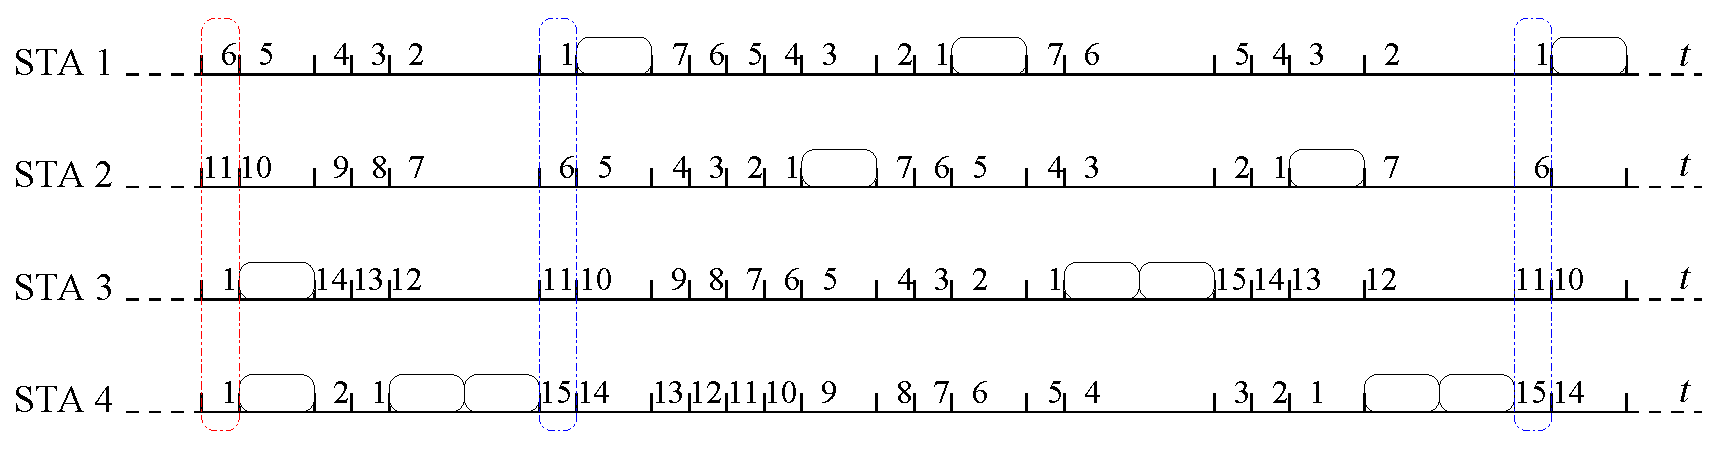
\includegraphics[width=0.8\linewidth]{figures/csma_eca_different_backoff_short.eps}
		\caption{An example of the temporal evolution of CSMA/ECA$_{\text{Hys+FS}}$ in saturation ($CW_{\min}=16$)}
		\label{fig:ECA+Hyst}
	\end{figure*}
	
	Algorithm~\ref{alg:fullECA} shows an implementation of CSMA/ECA$_{\text{Hys+FS}}$, while an example of CSMA/ECA$_{\text{Hys+FS}}$ with four contenders is shown in  Figure~\ref{fig:ECA+Hyst}. In the figure the first outline indicates a collision between STA-3 and STA-4, which will provoke an increment on both station's backoff stage ($k\leftarrow k+1$). Once STA-4's random backoff expires, CSMA/ECA$_{\text{Hys+FS}}$ instructs the station to transmit $2^{k}$ packets, and then use a deterministic backoff, $B_{\text{d}}=CW(k)/2$. The same behavior is followed by STA 3.
	
	With Hysteresis and Fair Share, CSMA/ECA$_{\text{Hys+FS}}$ is able to achieve greater throughput than CSMA/CA and for many more contenders, as shown in Figure~\ref{fig:ECA+H+F-throughput} extracted from~\cite{research2standards}. In the figure, the \emph{CSMA/ECA$_{\text{Hys+FS}}$} curve shows a greater throughput because collisions are eliminated and Fair Share allows nodes to send $2^{k}$ packets upon each transmission. This throughput increase is the result of aggregation via Fair Share, which also carries the effect of raising the average time between successful transmissions (see Section~\ref{timeBetweenSxTx}), which may affect delay-sensitive traffic, like gaming or live video/voice/tv streaming. \textcolor{red}{Channel errors or unsaturated traffic conditions will disrupt any collision-free schedule, generate collisions and push all stations's backoff stages to the maximum value very quickly (contributing to the delay increase). This issue is leveraged with Schedule Reset mechanims, presented in Section~\ref{schedReset}.}

	\begin{algorithm}[tb]
	\While{the device is on}
	{
	  $r \leftarrow 0$ ; $k \leftarrow 0$\;
	  $b \leftarrow \mathcal{U}[0,2^k\rm{CW}_{min}-1]$\;
	  \While{there is a packet to transmit}{
	    %\tcc{Initialize $a$.}
	    \Repeat{($r = R$) or (success)}{
	      %\tcc{First, backoff.}
	      \While{$B>0$}{
	        wait 1 slot\;
	        $B \leftarrow B-1$\;
	      }
	      \colorbox{yellow}{Attempt transmission of $2^k$ packets;}\\
	      \If{collision}{
	        %\tcc{Random backoff.}
	        $r \leftarrow r+1$\;
	        $k \leftarrow \min (k+1,m)$\;
	        $B \leftarrow \mathcal{U}[0, 2^k  \rm{CW}_{min} -1]$\;
	      }
	    }
	    $r \leftarrow 0$\;
	    %$s \leftarrow 0$\;
	    \eIf{success}{
	      %\tcc{Random backoff.}
	      \colorbox{yellow}{$B_{d} \leftarrow (2^{k}\rm{CW}_{min})/2-1$;}\label{backoffExample}\\
		$B \leftarrow B_{d}$;\\
	    }
	    {
	      Discard packet\;
	      $k \leftarrow 0$\; \label{labelReset}
	      $B \leftarrow \mathcal{U}[0, 2^k \rm{CW}_{min}-1]$\;
	    }
	  }
	  Wait until there is a packet to transmit\;
	}	
	\vspace{0.2cm}
	\caption{CSMA/ECA$_{\text{Hys+FS}}$}
	\label{alg:fullECA}
	\end{algorithm}


	\subsection{The effects of Aggregation}\label{effects-of-aggregation}
	Fair Share is an \textcolor{red}{A-MPDU} aggregation mechanism~\cite{A-MPDU} that coupled with the collision-free schedule built by CSMA/ECA$_{\text{Hys}}$ is able to provide short-term fairness. However, it also improves the throughput since the aggregation process makes the packet transmission more efficient by reducing overheads. The downside of Fair Share is that it may increase the time between two consecutive transmissions from the same node, which may affect negatively delay-sensitive applications such as gaming or high definition real-time video. \textcolor{red}{An example of the duration of a transmission, $T(l_{k})$, is provided by (\ref{eq:Ts}) in the following Section~\ref{ECA-bounds}.}
	
	In scenarios where short-term fairness and the time between consecutive transmissions are not relevant, Fair Share can be replaced by \emph{Maximum Aggregation} (MaxAg), which will significantly improve the system throughput. In Maximum Aggregation all nodes aggregate as many packets as possible at every transmission, i.e., they send $2^m$ packets in each attempt.

	Figure~\ref{fig:ECA-vs-DCF-maxAgg} shows the aggregated throughput for CSMA/ECA$_{\text{Hys+FS}}$, CSMA/ECA$_{\text{Hys+MaxAg}}$, CSMA/CA using the Fair Share mechanism (CSMA/CA$_{\text{FS}}$), and CSMA/CA$_{\text{MaxAg}}$. JFIs are shown below. Although CSMA/CA$_{\text{FS}}$ and CSMA/CA$_{\text{MaxAg}}$ perform aggregation, collisions degrade the aggregated throughput as more contenders attempt transmission. On the other hand, CSMA/ECA$_{\text{Hys+FS}}$ is able to build a collision-free schedule and takes advantage of the aggregation provided by Fair Share, which opposed to just using CSMA/ECA$_{\text{Hys+MaxAg}}$, it is fair.
	
	\begin{figure}[tb]
	\centering
		\includegraphics[width=0.7\linewidth,angle=-90]{figures/throughput-combined/throughput-combined-TON.eps}
		\caption{Throughput comparison~\cite{research2standards} (simulation parameters can be found in Section~\ref{simulations})}
		\label{fig:ECA+H+F-throughput}
	\end{figure}
	
	\begin{figure}[tb]
	\centering
		\includegraphics[width=0.7\linewidth,angle=-90]{figures/throughput-max-Ag/throughput-saturated-maxAgg-TON.eps}
		\caption{Throughput comparison with CSMA/CA$_{\text{MaxAg}}$: even though at low number of contenders CSMA/CA$_{\text{MaxAg}}$ achieves greater throughput than CSMA/ECA$_{\text{Hys+FS}}$, collisions eventually degrade the throughput below CSMA/ECA$_{\text{Hys+FS}}$'s when the number of contenders increases past $N=10$}
		\label{fig:ECA-vs-DCF-maxAgg}
	\end{figure}
	
	To summarise the effects of using aggregation:
	\begin{itemize}
		\item It increases the aggregated throughput: because nodes are able to send multiple packet in each attempt, the system throughput is increased. Moreover, Fair Share compensates those nodes at higher backoff stages to ensure throughput fairness.
		\item Maximum aggregation supposes the deactivation of the Fair Share mechanism: performing maximum aggregation upon each transmission attempt is equivalent to having different schedule lengths and not compensating nodes at higher backoff stages. Although the aggregated throughput increases, this results in an uneven distribution of the channel time among contenders, which renders it unfair.
		\item Longer periods between transmission attempts: given that each transmission takes longer, the time between transmission attempts also increases. This may specially affect delay-sensitive applications.
	\end{itemize}

	%\begin{figure}[tb]
%	\centering
%		\includegraphics[width=0.7\linewidth,angle=-90]{figures/fairness-max-Ag/fairness-maxAg-combined-TON.eps}
%		\caption{Fairness comparision when using maximum aggregation}
%		\label{fig:fairness-with-maximum-aggregation}
%	\end{figure}
	
	Since we consider that fairness and a short inter-transmission time are even more important than raw throughput for the next generation of WLANs, we keep CSMA/ECA$_{\text{Hys+FS}}$ as the reference protocol.
	
	\subsection{Throughput bounds of CSMA/ECA$_{\text{Hys+FS}}$}\label{ECA-bounds}
	
	They correspond to the maximum and minimum achievable throughput without the possibility of collisions using Hysteresis and Fair Share. The ideal CSMA/ECA$_{\text{Hys+FS}}$ network uses the minimum schedule length that guarantees a collision-free operation. That is, with a schedule length of $C=2^{k}B_{\text{d}}$, where $k = \left\lceil log_{2}(N/B_{\text{d}})\right\rceil$. Using this minimum schedule length, $N$ nodes will be at the same backoff stage if $N\leq B_{\text{d}}$. Otherwise, $h = N-(C-N)$ nodes would occupy the $k$-th backoff stage and the other $N-h$ \textcolor{red}{nodes the $(k-1)$-th one}. The system throughput is computed as follows:
	
	\begin{equation}
			S =
				\begin{cases}\label{eq:bound}
					hs_{k}(l_{k}) + (N-h)s_{k-1}(l_{k-1}), & \text{if } N > B_{\text{d}} \\
					Ns_{k}(l_{k}), & \text{otherwise}
				\end{cases}
	\end{equation}
	
	where $s_{k}(l_{k})$ and $s_{k-1}(l_{k-1})$ are the throughput achieved by the nodes at the $k$-th and $(k-1)$-th backoff stages sending $l_{k}$ and $l_{k-1}$ packets respectively. These are given by:
	
	\begin{subequations}
		\begin{align}
			&s_{k}(l_{k}) = \frac{l_{k} L}{hT(l_{k})+2(N-h)T(l_{k-1}) + \sigma_{e}(C - N)}\label{eq:HighNodes}\\
			&s_{k-1}(l_{k-1}) = \frac{l_{k-1} L}{(N-h)T(l_{k-1}) + k\frac{T(l_{k})}{2}}\label{eq:LowNodes}
		\end{align}
	\end{subequations}
	
	where $L$ is the data payload, $T(l_{k})$ and $T(l_{k-1})$ are the duration of the transmission of $l_{k}$ and $l_{k-1}$ packets, respectively; $\sigma_{e}$ is the duration of an empty slot. Additionally, $T(l_{k})$ derives from~(\ref{eq:Ts}):
	
	\begin{multline}\label{eq:Ts}
		T(l_{k})= \left( T_{\text{PHY}} + \left\lceil \frac{ \text{SF} + l_{k} (\text{MD}+\text{MH}+L) + \text{TB}}{L_{\text{DBPS}}}\right\rceil T_{\text{sym}} \right) \\ 
		+ \text{SIFS}+\left(T_{\text{PHY}} + \left\lceil\frac{\text{SF} + L_{\text{BA}} + \text{TB}}{L_{\text{DBPS}}} \right \rceil T_{\text{sym}} \right) + \text{DIFS} + \sigma_{e}
	\end{multline}
	
	where $T_{\text{PHY}}=32~\mu$s is the duration of the PHY-layer preamble and headers, $T_{\text{sym}}=4~\mu$s is the duration of an OFDM (Orthogonal Frequency Division Multiplexing) symbol. SF is the \emph{service field} ($16$ bits), $\text{MD}$ is the \textit{MPDU Delimiter} ($32$ bits), MH is the \emph{MAC header} ($288$ bits), TB is the number of \emph{tail bits} ($6$ bits), $L_{\text{BA}}$ is the \emph{Block-ACK} length ($256$ bits) and $L_{\text{DBPS}}=256$ is the number of bits in each OFDM symbol. SIFS, DIFS and $\sigma_{e}$ values can be found in Table~\ref{tab:mac-params}.

	The \emph{Lower-bound} is derived from considering the operation of an ideal CSMA/ECA$_{\text{Hys+FS}}$ network. Nodes use the minimum backoff stage possible and aggregate proportionally, thus yielding the minimum throughput achievable by a CSMA/ECA$_{\text{Hys+FS}}$ network. It is computed following~(\ref{eq:bound}) with $l_{k}=2^{k}$ and $l_{k-1}=2^{k-1}$.
	
	The \emph{Upper-bound} is obtained from considering the operation of a network using CSMA/ECA$_{\text{Hys+FS}}$, but forcing nodes to use the maximum backoff stage for determining the cycle length and the level of aggregation. It is also computed using~(\ref{eq:bound}) but considering that all nodes are in the maximum backoff stage ($k=m$) and therefore $l_{k}=2^{m}$.
	
	The maximum throughput achievable is the result of deactivating the Fair Share rules by forcing nodes to use maximum aggregation regardless of their backoff stage. This is called \emph{Maximum Aggregation (Hys+MaxAg)} in Figure~\ref{fig:ECA-bounds-comparison}. It can be derived from~(\ref{eq:bound}) considering $l_{k} = 2^{m}$ and $l_{k-1}=2^{m}$.
		
	It is interesting to see in Figure~\ref{fig:ECA-bounds-comparison} how collisions force colliding CSMA/ECA$_{\text{Hys+FS}}$ contenders to increase their backoff stage and aggregate more with Fair Share. This explains why the CSMA/ECA$_{\text{Hys+FS}}$ curve separates itself from the \emph{Lower-bound} at a very low number of contenders. 
	
	Although using maximum aggregation (see \emph{Maximum Aggregation (Hys+MaxAg)} curve in Figure~\ref{fig:ECA-bounds-comparison}) increases the throughput it carries the effect of unevenly distributing the available bandwidth among contenders, as mentioned in Section~\ref{effects-of-aggregation}.
	
	The tools for deriving these two curves are available as MATLAB functions in~\cite{ECA-bounds-example}. 
	
	\begin{figure}[tb]
	\centering
		\includegraphics[width=0.7\linewidth,angle=-90]{figures/throughput-w-model/throughput-combined-w-model-TON.eps}
		\caption{Upper and Lower throughput bounds for CSMA/ECA$_{\text{Hys+FS}}$}
		\label{fig:ECA-bounds-comparison}
	\end{figure}
	
	\subsection{Clock drift issue in descentralized collision-free MAC protocols}\label{clockDrift-issue}
	CSMA/ECA relies on stations being able to correctly count empty slots and consequently attempt transmissions in the appropriate slot according to the backoff timer. Failure to do so may be caused by clock imperfections inside the Wireless Network Interface Cards (WNIC), which is commonly referred to as \emph{clock drift}. As pointed out in~\cite{slotDrift}, clock drift is a common issue that degrades the throughput in distributed collision-free MAC protocols like the ones reviewed in Sect.~\ref{relatedWork}.
	
	While miscounting empty slots have no significant effect on CSMA/CA's throughput~\cite{slotDrift}, it has a direct impact on CSMA/ECA. In a collision-free schedule with saturated CSMA/ECA contenders, a station miscounting empty slots will \emph{drift} to a possibly busy slot, collide and force a re-convergence (if possible) to a collision-free schedule (see Sect.~\ref{performanceClockDrift}).
	
%	\textcolor{red}{\subsection{Real hardware implementation} 
%	Replacing the firmware of commercial WLAN cards with the Open Firmware for WiFi Networks, OpenFWWF~\cite{OpenFWWF}, allows the modification of time-sensitive operations in the MAC, like the backoff procedure. In Section~\ref{EDCA} we provide details regarding the tesbed, the firmware used and present results of real experiments using CSMA/ECA.}
%	

	\textcolor{red}{\subsection{Channel errors}}\label{errorEffect}
	Failed transmissions due to channel errors are handled as collisions by CSMA/ECA$_{\text{Hys+FS}}$. Therefore, collision-free schedules under this type of channel model are shorter. In order to accelerate the convergence to collision-free schedules after channel errors CSMA/ECA$_{\text{Hys+FS}}$ instruct nodes to \emph{stick} to the current deterministic backoff even after \emph{stickiness} number of consecutive failed transmissions. Stickiness is not a new concept to CSMA/ECA~\cite{barcelo2011tcf}, it allows for a faster convergence towards a collision-free schedule, especially when performing under heavy channel errors.
	
	Failed transmissions due to channel errors also means that a few moments of operation under a noisy channel can increase the contenders's deterministic backoff to its maximum value. Such event carries the undesired effects of increasing the time between successful transmissions, and a reduction in the overall system throughput due to shorter collision-free periods.
		
	\textcolor{red}{\subsection{Schedule Reset Mechanism}\label{schedReset}}
	CSMA/ECA$_{\text{Hys+FS}}$ instructs nodes to keep their current backoff stage after a successful transmission (resetting it to zero only if reaching the retransmission attempt limit, see line~\ref{labelReset} in Algorithm~\ref{alg:fullECA}). This is done in order to increase the cycle length and provide a collision-free schedule for many contenders, which is desirable in dense scenarios.
	
	Nevertheless, having a big deterministic backoff increases the time between successful transmissions. Furthermore, if not operating in a scenario with many nodes the empty slots between transmissions are not longer negligible and degrade the overall throughput of the system. For instance, if nodes withdraw from the contention their previously used slots will now be empty. On the other hand, in scenarios with channel errors contenders rapidly end up with the largest deterministic backoff. Nodes should be aware of this issue and pursue opportunities to reduce their deterministic backoff, $B_{\text{d}}$ without sacrificing too much in collisions. 
	
	The \emph{Schedule Reset} mechanism for CSMA/ECA$_{\text{Hys+FS}}$ consists on finding the smallest collision-free schedule (if any) between a contender's transmissions and then change the node's deterministic backoff to fit in that schedule. Take a contender with $B_{\text{d}}=32$ as an example. By listening to the slots between its transmissions, it is possible to determine the availability of smaller (and possibly) collision-free schedules.
	
	Figure~\ref{fig:scheduleReset1} shows the slots between the transmissions of a contender with $B_{\text{d}}=32$. Starting from the left, the current $B_{\text{d}}=0$ means that the first slot will be filled with the contender's own transmission. Each following slot containing either a transmission or a collision is identified with the number one, while empty slots are marked with a zero. Notice that the highlighted empty slots appear every eight slots, suggesting that a schedule reduction from $B_{\text{d}}=32$ to $B_{\text{d}}^{*}=8$ is possible\footnote{$B_{\text{d}}=2^{0}CW_{\min}/2=8$ (see Table~\ref{tab:mac-params}). So the change is made to the backoff stage, $k$. In this case from $2$, to $k=0$. This means that any new schedule must also be a power of two.}. The schedule change is performed after the contender's next successful transmission.
	
	%, coupled with an increase by one in the node's \emph{stickiness}~\cite{L_MAC2}. 
	%\footnote{Trailing waiting periods, like the SIFS, are composed of empty slots. These allow nodes to decrement their backoff counters even after a collision or successful slots. Without loss of generality, the stations in our examples and simulations decrement their respective backoff counters by one after these kind of slots (see example in Figures~\ref{fig:ECA} and~\ref{fig:ecaQoS}).}
		\begin{figure}[tb]
		\centering
			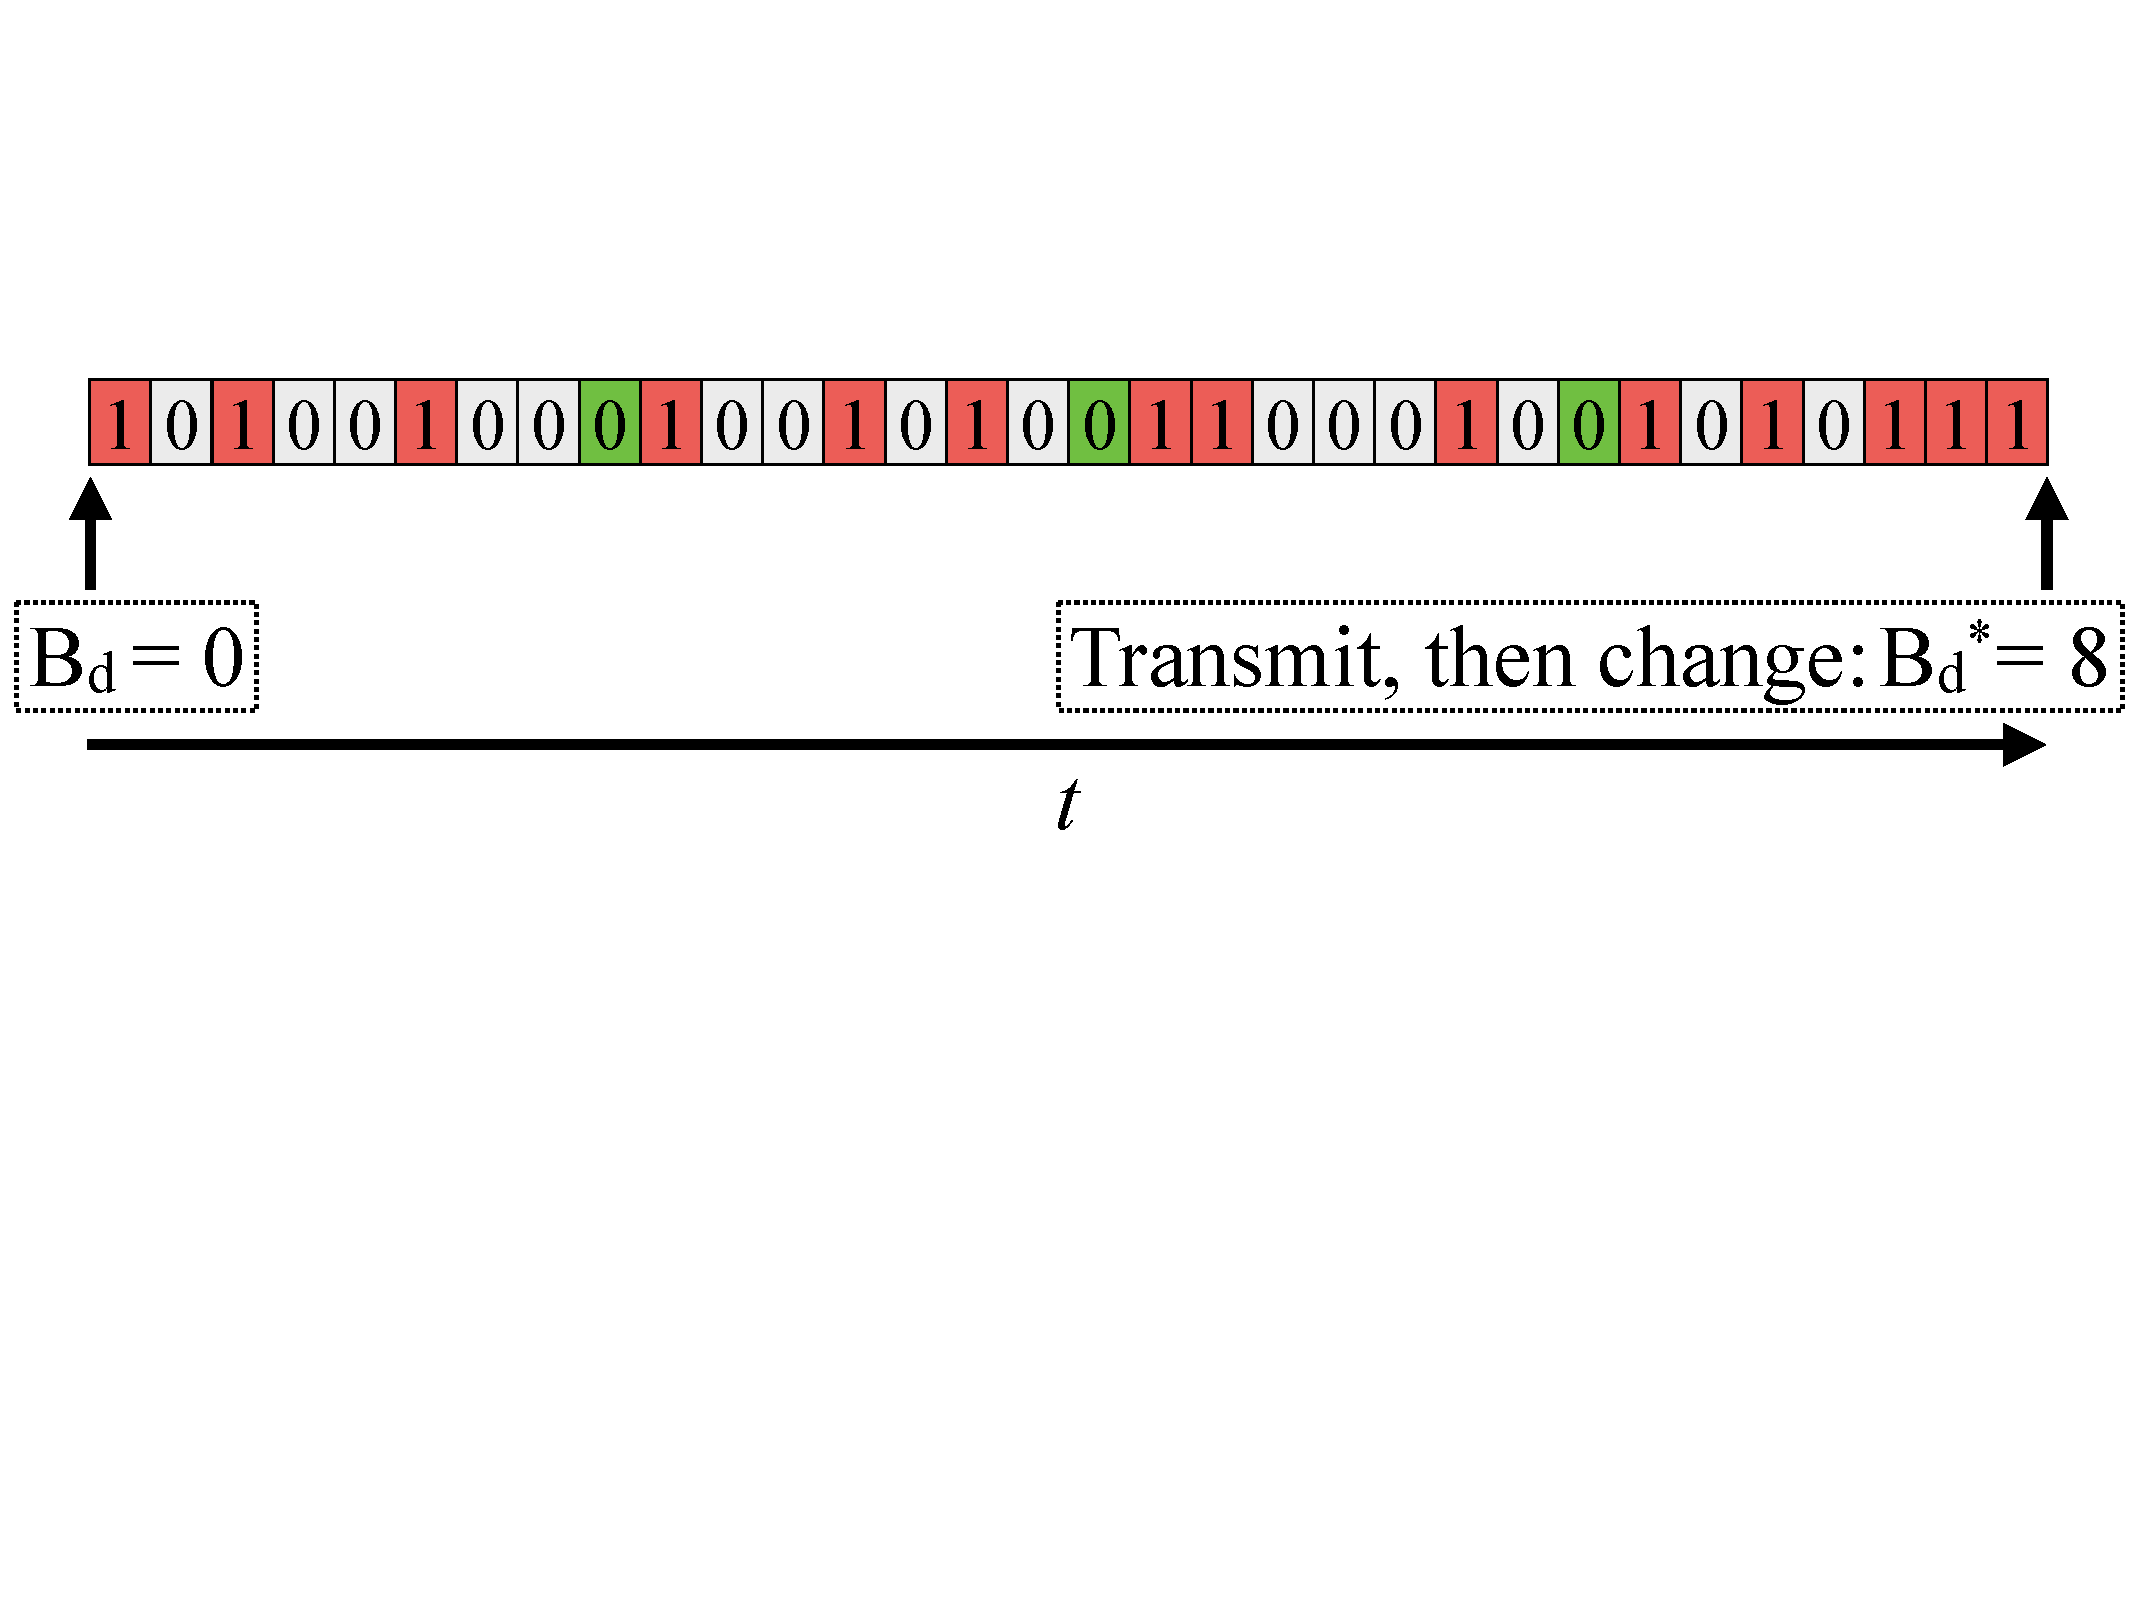
\includegraphics[width=\linewidth]{figures/tonFigs/scheduleReset.pdf}
			\caption{Example of the Schedule Reset mechanism.}
			\label{fig:scheduleReset1}
		\end{figure}
		
		
			\begin{algorithm}[tb]
		\If{sxTx == 1}{
			Initialising\;
			\If{B == 0}{
				$b~[B_{\text{d}}] = \{0\}$\;
				$t = 0$\;
			}
		}
		\If{(sxTx $>$ 0) \&\& (sxTx $\leq~\gamma$)}{
			Filling the bitmap\;
			$b[t] \|\sigma_{i}(t)$\label{bitwiseOR}\;
			$t++$\;
			\If{$t == B_{\text{d}} -1$}{
				$t=0$\;
			}
		}
		\If{sxTx == $\gamma$}{\label{evaluations}
			Analising\;
			sxTx = $0$\;
			\For{($j=0;~j<k;~j++$)}{\label{sets}
				$y=2^{j}CW_{\min}/2$\;
				isItPossible $= 0$\;
				\For{($m=y;~m<B_{\text{d}};~m+=y$)}{
					isItPossible$~+=b[m]$\;\label{filling}
				}
				\If{isItPossible == $0$}{\label{testFilling}
					change = $1$\;
					newStage = $m$\;
					{\bf break};
				}
			}
		}
		\If{change == $1$}{
			Making the change\;
			$k$ = newStage\;
			change = $0$\;\label{endAssignment}
		}
		\vspace{0.2cm}
		\caption{Schedule Reset Mechanism for CSMA/ECA$_{\text{Hys+FS}}$. Every consecutive successful transmission increases the variable SxTx by one, while a collision resets it to zero. The algorithm is called a \emph{reset} when all smaller deterministic backoff are tested. On the other hand, when $j$ in line~\ref{sets} is initialised to $j=k-1$, it is called a schedule \emph{halving}}\label{alg:schedRest}
	\end{algorithm}
		
		
		\subsubsection{Keeping collision-free schedules}
		Schedule Reset is described in Algorithm~\ref{alg:schedRest}. Each contender starts filling a bitmap $b$ of size $B_{\text{d}}$ with the information observed in each passing slot during $\gamma=B_{\text{d}}/C$ consecutive successful transmissions (sxTx in Algorithm~\ref{alg:schedRest}); where $C=2^{m}CW_{\min}/2$ is the biggest deterministic backoff, and $\gamma$ is referred to as the Schedule Reset \emph{threshold} from this point forward.
		
		Each bit $t,~t\in\{0,\ldots ,B_{\text{d}}-1\}$ in the bitmap is the result of a bitwise OR operation between its current value and the state of the corresponding slot. This is shown in Line~\ref{bitwiseOR} in Algorithm~\ref{alg:schedRest}, where $\sigma_{i}(t)$ is a function that evaluates to $0$ if the slot corresponding to $b[t]$ is empty in iteration $i$, $i \in\{1,\ldots,\gamma\}$; or $1$ otherwise. After $\gamma$ iterations, the bitmap is evaluated (line~\ref{evaluations} in Algorithm~\ref{alg:schedRest}).
		
	%	After $\gamma$ iterations the bitmap is evaluated.
		
	%	\begin{equation}
	%		\sum\limits_{t\in A} b[t] =
	%				\begin{cases}\label{eq:schedEval}
	%					0, &\text{make change} \\
	%					>0, &\text{discard}
	%				\end{cases}
	%	\end{equation}
		
		Schedule Reset tests all possible deterministic backoffs that are smaller than the current $B_{\text{d}}$ (lines~\ref{sets}-\ref{filling} in Algorithm~\ref{alg:schedRest}), starting with the smallest one. If the corresponding bits in the bitmap are registered as empty, the process is stopped and the change to the new deterministic backoff is made (lines~\ref{testFilling}-\ref{endAssignment} in Algorithm~\ref{alg:schedRest}). Otherwise, the process is restarted after the next successful transmission.
		
		Using Figure~\ref{fig:scheduleReset1} as an example, we can see that the sum $\sum\limits_{t} b[t]=0$, for $t\in\{8,16,24\}$. This means that the transmission slots corresponding to a deterministic backoff, $B^{*}_{\text{d}}=8$ are free, therefore a change of schedule is possible. In case of suffering a collision immediately after applying the schedule reduction, the node reverses the changes made by Schedule Reset before handling the collision.
		
		%In (\ref{eq:schedEval}), the set $A$ contains all possible shorter schedule lengths, e.g.: $A\in\{2^{j}CW_{\min}/2,\ldots, 2^{k-1}CW_{\min}/2\}$, for $j\in[0,\ldots,k-1]$. 
	
		\subsubsection{Facing channel errors}\label{aggr}
		
		the default $\gamma$ ensures that the bitmap registers all the transmission slots in the network (assuming saturated traffic and a perfect channel), providing enough information for performing the schedule reduction without disrupting collision-free schedules. 
		
		Nevertheless, this $\gamma$ can be rendered too conservative when in the presence of channel errors. This condition produces Schedule Reset bitmaps that do not contain enough information for successfully avoiding collisions after the schedule reduction. This is also true for any $\gamma^{*}>\gamma$.
		
		This effect is leveraged by setting $\gamma=1$, meaning that the bitmap is filled with the information of slots between only two consecutive transmissions. This measure increases the frequency of schedule reset attempts.
		%Further, there is the option of doing a schedule \emph{halving}. That is, with a set $A\in\{2^{k-1}CW_{\min}/2\}$.
	%	
	%	Schedule Reset can also be configured to increase the node's \emph{stickiness} after a successful reduction of the schedule. Stickiness is not a new concept to CSMA/ECA~\cite{barcelo2011tcf}. It simply instructs the contender to \emph{stick} to the deterministic backoff even in the event of \emph{stickiness} number of consecutive failed transmissions. This allows for a faster convergence towards a collision-free schedule, especially when performing under heavy channel errors. 
	%	
	
	\subsection{Backwards compatibilty and coexistence}
	CSMA/ECA$_{\text{Hys+FS}}$ springs from a modification to CSMA/CA's backoff mechanism. It keeps the range of values CSMA/CA nodes use to draw a random backoff (i.e., use the same $CW_{\min}$ and $CW_{\max}$), allowing CSMA/ECA$_{\text{Hys+FS}}$ contenders to coexist with CSMA/CA nodes in the same network. Further, the selection of CSMA/ECA$_{\text{Hys+FS}}$'s deterministic backoff, $B_{\text{d}}$, is the expected value for the current backoff stage $k$ ($B_{\text{d}}\coloneqq\lceil{E[0,CW(k)]}\rceil$)~\cite{research2standards}, which ensures fairness among contenders. An overview of the attained throughput for different proportions of CSMA/ECA$_{\text{Hys+FS}}$ and CSMA/CA nodes is presented in Section~\ref{coexistance-w-csmaca}.
	
	